\documentclass[14pt]{extreport}
\usepackage{listings}
\usepackage[english]{babel}
\usepackage[utf8]{inputenc}
\usepackage{amsmath}
\usepackage{graphicx}
\usepackage{textcomp}
\usepackage{qtree}
\usepackage[colorinlistoftodos]{todonotes}
\usepackage {tikz}
\usetikzlibrary {positioning}
%\usepackage {xcolor}
\definecolor {processblue}{cmyk}{0.96,0,0,0}
\usepackage{listings}
\lstset{language=C, tabsize=4, mathescape}
\usepackage{tikz}
\usetikzlibrary{calc,shapes.multipart,chains,arrows}

\usepackage{geometry}
\geometry{legalpaper, margin=1in}

\def\codefont{
  
  \fontsize{13pt}{13pt}\selectfont}
\definecolor{codebgcolor}{HTML}{EDEDED}
\newenvironment{code}
{\begin{center}
    \begin{tikzpicture}
      \node [fill=codebgcolor,rounded corners=5pt]
      \bgroup
      \bgroup\codefont
      \begin{tabular}{l}}
      {\end{tabular}
      \egroup
      \egroup;
    \end{tikzpicture}
  \end{center}}


\title{Algorithm Engineering}

\author{Luca Corbucci}

\date{\today}

\begin{document}
\maketitle

\tableofcontents

\chapter{Lezione 1}

\section{Definizione di algoritmo}

Nel libro "The Art of Computer Programming" Donald Knuth definisce un algoritmo come "una procedura finita, definita, effettiva con alcuni output". Nel dettaglio:
\begin{itemize}
    \item Finita: l'algoritmo deve terminare sempre dopo un numero ragionevole di passaggi. Il termine "ragionevole" (rispetto alla difficoltà del problema) è legato all'efficienza dell'algoritmo;
    \item Definito: ogni step dell'algoritmo deve avere un significato preciso e non ambiguo, se lo legge un'altra persona non deve avere una "interpretazione" diversa dalla nostra;
    \item Effettivo: tutte le operazioni effettuate nell'algoritmo devono essere abbastanza semplici da poter essere eseguite anche con carta e penna.
\end{itemize}

\section{Un nuovo modello}

Un algoritmo va analizzato per capire il tempo e lo spazio necessario per la sua esecuzione, il modello basilare che si è considerato fino a qualche anno fa è il "RAM Model" (1 CPU + 1 Memoria) in cui ogni accesso alla memoria costa $O(1)$ e il tempo necessario $T(N)$ lo calcoliamo considerando il numero di operazioni che vengono svolte dall'algoritmo. Spazio e tempo dipendono dalla $n$ in input, maggiore è n e più aumentano gli step necessari per l'esecuzione dell'algoritmo (e quindi il tempo), allo stesso modo aumentano anche le celle di memoria occupate durante l'esecuzione dell'algoritmo (e quindi lo spazio necessario).
Dati due algoritmi analizzati con il modello RAM è possibile confrontarli per capire quale dei due è migliore dal punto di vista del tempo necessario all'esecuzione.

Il modello RAM attualmente non è più utilizzato (se non in teoria) e si è passati ad un modello più complicato in cui abbiamo più di una CPU e una gerarchia di memoria. L'accesso alla memoria ha un costo differente a seconda di dove si trova la memoria all'interno della gerarchia, alla cache si accede in poco tempo (nanosecondi), al disco si accede in un tempo che è nell'ordine dei millisecondi. 
Per risolvere questo problema di "I/O Bottleneck" o si cerca di trovare soluzioni hardware o si migliorano gli algoritmi, spesso migliorando gli algoritmi si ottiene una soluzione migliore rispetto al miglioramento dell'hardware.
Ad esempio, consideriamo 3 algoritmi con 3 costi differenti in termini di tempo necessario per l'esecuzione:
\begin{itemize}
    \item $C_1(n) = n$: se abbiamo un tempo massimo $t$ e ogni operazione di $I/O$ costa c, i dati su cui possiamo lavorare sono al massimo $n*c = t$ ovvero $n = \frac{t}{c}$. Se aumentiamo il tempo di k, la quantità di dati scala perfettamente di un fattore k. $n = \frac{t*k}{c}$.
    \item $C_2(n) = n^2$: se abbiamo un tempo massimo $t$ e ogni operazione di $I/O$ costa c, i dati su cui possiamo lavorare sono al massimo $n^2*c = t$ ovvero $n = \sqrt{\frac{t}{c}}$. Se aumentiamo il tempo di k, la quantità di dati diventa. $n = \sqrt{\frac{t*k}{c}}$.
    \item $C_3(n) = 2^n$: se abbiamo un tempo massimo $t$ e ogni operazione di $I/O$ costa c, i dati su cui possiamo lavorare sono al massimo $2^n*c = t$ ovvero $n = log(\frac{t}{c})$. Se miglioriamo l'hardware e il tempo aumenta di k, la quantità di dati non scala. $n = log(\frac{t*k}{c})$.
\end{itemize}

Quindi il miglioramento dell'hardware non sempre porta un miglioramento in termini di tempo necessario per l'esecuzione degli algoritmi e molto spesso è preferibile avere un algoritmo migliore.

\section{Un primo problema: sommare gli elementi di un array}

Consideriamo il problema di dover sommare tutti gli n elementi di un array.
Banalmente possiamo scorrere l'array e sommare in una variabile i vari elementi, eseguiamo n somme.
Possiamo generalizzare questo approccio considerando un modo differente di accedere agli elementi dell'array, consideriamo infatti due parametri b = dimensione del blocco logico dell'array tale che per ogni blocco $[0,n/b]$ abbiamo che il blocco j comprende gli elementi $A_j = A[j*b+1,(j+1)*b]$ e s = numero di salti da fare verso destra una volta letto un elemento dell'array, s deve essere coprimo con $n/b$ perchè altrimenti andiamo a vedere sempre gli stessi blocchi. Otteniamo un modello $A_{s,b}$ per l'accesso ai dati dell'array, indipendentemente dai parametri s e b, da un punto di vista computazionale, tutti l'algoritmo ha sempre lo stesso costo perchè leggiamo sempre n interi, la differenza ce l'abbiamo in quanto ad efficienza se la dimensione n dell'array cresce perchè quando cresce n ed aumentano i dati da sommare, questi saranno distribuiti su tanti livelli di memoria e quindi avremo un costo maggiore per accedere ai vari livelli. Se ad esempio abbiamo D dischi e in ogni disco vogliamo accedere ad una pagina di memoria di dimensione B allora leggeremo un totale di $D*B$ elementi provenienti da D dischi differenti.
Per migliorare l'efficienza dell'algoritmo nel momento in cui si accede ai dati in memoria quindi devono essere sfruttate principalmente due feature:
\begin{itemize}
\item Località spaziale: se accedo il blocco I è probabile che poi accederò anche il blocco I+1; 
\item Località temporale: se ora accedo ad un certo blocco, è probabile che lo accederò di nuovo a breve.
\end{itemize}

Analizziamo l'algoritmo $A_{s,b}$ considerando un array di n elementi, dei blocchi logici nell'array di b elementi e delle pagine di memoria grandi B.
\begin{itemize}
\item Consideriamo $A_{1,1}$ quindi abbiamo pagine logiche grandi 1 elemento e saltiamo ogni volta di 1, quindi in pratica scorriamo l'array. L'algoritmo svolge $\frac{n}{B}$ operazioni di I/O.
\item Prendiamo il caso in cui $b<B$ e s = 2 ovvero ogni volta saltiamo un elemento del blocco b. Se ad esempio abbiamo b=2 e B=4 vuol dire che ogni volta consideriamo solamente due elementi del blocco B quindi poi è necessario caricare due volte il blocco in memoria per accedere di nuovo agli elementi che non abbiamo ancora visto.
Quindi le operazioni di I/O diventano in questo caso $\frac{2*n}{B}$.
\end{itemize}
Generalizzando questo ragionamento possiamo dire che il costo delle operazioni di I/O dipende dalla scelta di s e quindi sarà $\frac{s*n}{B}$.

Consideriamo ora il costo complessivo dell'esecuzione dell'algoritmo andando a considerare lo step di computazione e lo step di accesso alla memoria.
Consideriamo che lo step di accesso alla memoria è necessario perchè abbiamo una memoria interna di dimensione M ma i dati che vogliamo prendere in considerazione sono $(1+\epsilon )*M$ ovvero rimangono fuori dalla memoria interna $\epsilon * m$ elementi.
Consideriamo inoltre la probabilità di un fault di I/O ovvero la probabilità di dover andare in memoria per prendere i dati necessari:
\begin{itemize}
\item Se $p(\epsilon) = 1$ accedo sempre al disco
\item Se $p(\epsilon) = 0$ non accedo mai al disco
\item Se $p(\epsilon) =\frac{\epsilon}{1+\epsilon}$ allora l'accesso al disco è completamente random. 
\end{itemize}
Ogni step dell'algoritmo ha un costo di:
\begin{equation}
1*P(Computational Step) + t_m * P(Memory access step)
\end{equation}
Dove con probabilità A eseguo lo step di memory access e con probabilità (1-A) l'altro tipo di step.
Dove $t_m$ viene calcolato come la somma della probabilità di un accesso in memoria interna e un accesso al disco:
\begin{equation}
T_m = 1*(1-p(\epsilon)) + c*p(\epsilon)
\end{equation}
Dove c è il costo dell'accesso al disco.

Anche se sfruttiamo i principi di località, gli accessi al disco hanno un costo molto alto e comportano dei problemi perchè vanno a rallentare l'esecuzione dell'algoritmo. Aumentando la N questo problema si nota ancora di più perchè aumentano i livelli di memoria in cui vengono posizionati i vari elementi dell'array.

\chapter{Lezione 2: Maximum Sub-Array Sum}

Consideriamo il problema del Maximum Sub-Array Sum, dato un array con N elementi dove possono essere presenti sia numeri positivi che negativi vogliamo calcolare il sub-array di somma massima ovvero vogliamo trovare le posizioni (b,s) che indicano l'inizio e la fine del sub-array.
Se l'array fosse solamente con numeri positivi potremmo restituire subito tutto l'array, se fossero solamente negativi potremmo restituire il valore più alto. 
Esistono varie soluzioni per risolvere questo problema, da alcune più banali a quella lineare, in tutti i casi abbiamo in comune il costo delle operazioni I/O da effettuare che sono sempre $O(n/B)$ perchè in ogni caso dobbiamo vedere tutti gli elementi dell'array e quindi accederò in memoria sempre almeno $n/B$ volte, indipendentemente dalla dimensione di B. Questa proprietà è detta di cache-oblivious.
Esempio: Abbiamo l'array $A = [4,-6,3,1,3,-2,3,-4]$ e il sub array di somma massima è $[3,1,3]$. Nella soluzione non è detto che ci siano solamente numeri positivi, possono anche essercene di negativi.

\section{Algoritmo cubico per risolvere il problema}

Una prima soluzione consiste nell'utilizzo di un algoritmo cubico per risolvere il problema, la complessità in termini di tempo è quindi $O(n^3)$:


\begin{code}
\begin{lstlisting}[escapeinside={(*}{*)}]
MaxSum = - $\infty$
for(b = 1; b<n; b++) do
    for(s=b; s<n; s++) do
        TmpSum = 0
        for(i=b; i<s; i++) do
            TmpSum += D[i];
        end for
        if(MaxSum < TmpSum) then
            MaxSum = TmpSum;
            $b_0$ = b;
            $s_0$ = s;
        end if
    end for
end for
return MaxSum, $b_0$, $s_0$
\end{lstlisting}
\end{code}

L'upper bound è $O(n^3)$ perchè non possiamo generare più di $\frac{n^2}{2}$ coppie di n elementi, il lower bound è $\Omega(n^3)$.

\section{Algoritmo quadratico}

Il problema dell'algoritmo cubico sta nel terzo for che va a sommare di nuovo il sub-array ogni volta che cambia la s del secondo for. Quindi in pratica faccio ogni volta da 0 la somma del sotto array A[b,s] quando invece basterebbe solamente aggiungere l'elemento A[s+1] nel momento in cui aumenta il valore di s.
Si passa quindi ad una soluzione più efficiente:

\begin{code}
\begin{lstlisting}[escapeinside={(*}{*)}]
MaxSum = - $\infty$
for(b = 1; b<n; b++) do
    TmpSum = 0
    for(s=b; s<n; s++) do
        TmpSum += D[s];
        if(MaxSum < TmpSum) then
            MaxSum = TmpSum;
            $b_0$ = b;
            $s_0$ = s;
        end if
    end for
end for
return MaxSum, $b_0$, $s_0$
\end{lstlisting}
\end{code}

Il costo in questo caso è $O(n^2)$ questo perchè il numero delle somme che vengono svolte è pari a:
\begin{equation}
    \sum^n \limits_{b=1} (1+\sum^n \limits_{s=b} 1) =  \sum^n \limits_{b=1} (1+(n-b+1)) = \sum^n \limits_{b=1} (2+n-b)) =
\end{equation}
\begin{equation}
    = n * (2+n) - \sum^n \limits_{b=1} b = n^2 + 2n - \frac{n(n-1)}{2} = O(n^2)
\end{equation}

\section{Algoritmo lineare}

Esiste un algoritmo lineare che quindi funziona in tempo $O(n)$ e che risolve il problema.
L'algoritmo in questione si basa su due proprietà, preso il sub-array di somma massima $A[b_0,s_0]$:
\begin{itemize}
    \item La somma degli elementi presenti prima dell'elemento $b_0$ è minore di 0, altrimenti la inseriremmo nel sub array di somma massima. Quindi abbiamo che la somma di $A[x,b_0] < 0$.
    \item Il primo elemento (e anche il prefix array) dell'array di somma massima non può essere minore di 0 altrimenti potremmo togliere l'elemento e avere una somma maggiore. Quindi abbiamo che la somma $A[b_0,y] > 0$ con $y<s_0$.
\end{itemize}

Sfruttando queste due proprietà si ottiene il seguente algoritmo:

\begin{code}
\begin{lstlisting}
MaxSum = -$\infty$
TmpSum = 0
b = 1;
for(s=1; s < n; s++) do
    TmpSum += D[s];
    if(MaxSum < TmpSum) then
        MaxSum = TmpSum
        $b_0$ = b
        $s_0$ = s
    end if
    if(TmpSum < 0) then
        TmpSum = 0
        b = s+1
    end if
end for
return MaxSum, $b_0$, $s_o$
\end{lstlisting}
\end{code}

Dato che ogni elemento viene analizzato solamente una volta, il costo in termini di tempo è $O(n)$, bisogna però dimostrare la correttezza dell'algoritmom per farlo si deve dimostrare che valgono le due proprietà elencate in precedenza:
\begin{itemize}
    \item Quando TmpSum è minore di 0 abbiamo un reset del valore di b che diventa uguale a $s+1$. In questo modo vale la prima proprietà;
    \item Quando troviamo che la TmpSum non è minore di 0 non modifico la b, quindi vale anche la seconda proprietà perchè vuol dire che il prefix dell'array è maggiore di 0.
\end{itemize}

L'algoritmo è cache-oblivious perchè indipendentemente dalla dimensione B della pagina che copio in memoria, il numero delle operazioni di I/O rimane sempre $n/B$.

\section{Un altro algoritmo lineare}

Esiste un altro algoritmo lineare per risolvere il problema delle Maximum Sub-Array sum, in questo caso sfruttiamo la seguente proprietà:
\begin{equation}
    max_s max_{b<s} Sum_D[b,s] = max_s max_{b<s}(Sum_D[1,s]-Sum_D[1,b-1])
\end{equation}

Ovvero andiamo a calcolare la somma di tutti gli elementi presenti nel sub-array D[1,S] e poi però sottraiamo gli elementi che non fanno parte del sub-array con somma maggiore.
Per eseguire questo calcolo abbiamo bisogno di alcuni array ausiliari:
\begin{itemize}
    \item Utilizziamo un array P in cui salviamo le somme prefisse calcolate partendo dall'array D di partenza. Questo calcolo lo svolgiamo scorrendo una sola volta l'array D e inserendo in P ogni volta la somma di $P[i]=P[i-1]+D[i]$. 
    Una volta ottenuto l'array P possiamo riscrivere il problema come:
    \begin{equation}
    max_s max_{b<s}(P[s]-P[b-1]) = max_s(P[s] - min_{b<s} P[b-1])
    \end{equation}
    \item Un array M con i minimi che troviamo all'interno dell'array P. Per riempire questo array scorrendo solamente una volta D dobbiamo calcolare: $M[i] = min{M[i-1],P[i]}$. Quindi possiamo nuovamente scrivere la formula per il calcolo del Maximum Sub-array sum come:
    \begin{equation}
    max_s (P[s]-M[s-1])
    \end{equation}
\end{itemize}

\begin{code}
\begin{lstlisting}
def MaximumSubArray(array):
    n = len(array)
    MaximumSum = -9999999
    minTmpSum = 0
    TmpSum = 0
    b0 = 0
    b = 0
    s0 = 0

    for i in range(0,n):
        TmpSum += array[i]

        if(MaximumSum < TmpSum - minTmpSum):
            MaximumSum = TmpSum - minTmpSum
            b0 = b
            s0 = i
        
        if(TmpSum < minTmpSum):
            minTmpSum = TmpSum
            b = i+1

    return MaximumSum, b0, s0

testArray = [4,-6,3,1,3,-2,3,-4,1,-9,6]
print MaximumSubArray(testArray)
\end{lstlisting}
\end{code}

\section{Varianti per il problema}

Il problema della Maximum sub-array sum può essere adattato anche alla bio informatica, in questo caso però non si ha un sub-array ma un segmento (ad esempio di DNA) in cui abbiamo una sequenza di lettere A,T,G,C con l'obiettivo di trovare i segmenti che hanno il maggior numero di G e C.
Ci sono due approcci al problema:
\begin{itemize}
    \item Assegnamo un valore $p$ a T e A, un valore $1-p$ a G e C. In questo modo data una sequenza lunga l abbiamo un calcolo complessivo di $x-p*l$.
    \item Assegnamo valore 0 alle lettere T e A, valore 1 alle lettere G e C. Complessivamente il calcolo, dato un segmento lungo l diventa $\frac{x}{l}$ dove x è il numero delle occorrenze di G e C.
\end{itemize}

Assumiamo di voler risolvere il seguente problema:
\newline
"Dato un array D[1,n], trovare il segmento più lungo la cui somma degli elementi produce una densità maggiore di un certo valore t".
\newline
Con una riduzione possiamo passare da un problema in cui si cerca un segmento la cui somma è maggiore di t ad un problema in cui si cerca il segmento in cui valore la proprietà:
\begin{equation}
    \sum^y \limits_{k=x} (D[k]-t) \geq 0
\end{equation}

Il procedimento è induttivo:
\begin{itemize}
    \item Ad ogni step dell'algoritmo $i=1,2,...n$, ci troviamo ad avere una possibile soluzione formata dal segmento $D[l_{i-1}, r_{i-1}$, allo step $i$ abbiamo due possibilità. O la nuova soluzione non migliora il precedente risultato, quindi manteniamo come risultato il segmento $D[l_{i-1}, r_{i-1}$ che quindi diventa $D[l_{i}, r_{i}$ oppure andando avanti di un elemento abbiamo un segmento più lungo del precedente quindi $r_i = i$.
    \item Se abbiamo il caso $r_i = i$ e quindi il segmento $D[l_i, r_i]$ è più lungo del precedente abbiamo in particolare che l'indice $l_i$ occorre a sinistra della posizione $L_i = i - (r_{i-1} - l_{i-1}$ (perchè il segmento $D[l_i, r_i]$ deve essere più lungo del precedente) e questo mi dice che la $l_i$ si trova a sinistra di $L_i$.
    \item Dobbiamo quindi trovare il più piccolo indice $l_i$ tale che $l_i \in [1,L_i)$ e tale che la somma del segmento $D[l_i,i] \geq t$.
    Vogliamo trovare l'indice $l_i$ più piccolo a sinistra di $L_i$ perchè vogliamo trovare il segmento più lungo.
\end{itemize}

Il problema diventa quindi:
\newline
"Trovare l'indice $l_i$ più piccolo nell'intervallo $[1,L_i]$ tale che $Sum_D[l_i,i] \geq t$"
\newline

Possiamo esprimere il problema utilizzando l'array con le somme prefisse P che abbiamo già usato in precedenza:
\begin{equation}
    Sum_D[1,i] - Sum_D[1, l_{i} - 1] = P[i] - P[l_i - 1] \geq t
\end{equation}

La $l_i$ deve essere un indice X che sia presente all'interno dell'intervallo $1,L_i$ tale che vale $P[i]-P[x] \geq t$.
Dato che per motivi di efficienza non possiamo scorrere tutta la sequenza di elementi compresi tra 1 e $L_i$ dobbiamo trovare una soluzione migliore.
Per ogni iterazione i:
\begin{itemize}
    \item Calcoliamo $C_{i,j}$ ovvero calcoliamo il minimo più a sinistra presente all'interno dell'intervallo $P[1,C_{i,j-1} - 1]$
    \item Per j che cresce abbiamo una cosa del genere: $C_{i,0} = L_i $ è in posizione 8 (ovvero un dummy value all'inizio), poi si calcola $C_{i,1} = leftmost min(P[1,8-1])$ quindi, ad esempio $C_{i,1} = 1 $.
\end{itemize}

Ora data la definizione, valgono alcune proprietà:
\begin{itemize}
    \item Andando avanti con le iterazioni, l'indice j di $C_{i,j}$ si sposta sempre più a sinistra
    \item Andando avanti con le iterazioni i valori di $P[C_{i,j}]$ sono sempre maggiori
    \item Il valore $P[C_{i,j}]$ è minore di tutti i valori che sono presenti alla sua sinistra
\end{itemize}

Conoscendo queste proprietà possiamo dire che:
\newline
Ad ogni iterazione i, l'indice più grande j* tale che $Sum_D[C_{i,j},i] \geq t$ ci restituisce il segmento più lungo che stiamo cercando. L'indice j* è quello che troviamo più a sinistra nell'array P, ad ogni passo in cui modifichiamo la $r_i$ viene calcolato un j più a sinistra.
\newline

Sapendo che $Sum_D[C_{i,j},i]$ la possiamo riscrivere come $P[i] - P[C_{i,j]}$ possiamo dire che tutti i segmenti nell'intervallo $D[z,i]$ con $z<C_{i,j}$ hanno somma minore di $Sum_D[C_{i,j},i]$.

Per il calcolo efficiente di $l_i$ dobbiamo considerare altri due calcoli:
\begin{itemize}
    \item Come calcoliamo $C_{i,j}$ quando la i aumenta? Dato che $C_{i,j}$ dipende solamente da $C_{i-1,j-1}$ allora possiamo considerare un array LMin in cui salviamo in posizione $LMin[L_i]$ la posizione del minimo più a sinistra nell'intervallo $P[1,i-1]$. 
    Quindi abbiamo che $C_{i,1} = LMin[L_i]$ e in generale $C_{i,k} = LMin^k[L_i]$.
    Il calcolo di LMin[x] viene svolto in tempo costante perchè il valore corrispondente è il minimo tra LMin[x-1] e P[x-1]. 
    \item Dobbiamo cercare l'indice j* in tempo costante. Se consideriamo che allo step i dobbiamo svolgere un numero $s_i > 1$ di step per calcolare j*, possiamo subito dire che aggiungiamo al costo dell'algoritmo un costo $O(s_i)$. Sapendo che il segmento completo non può essere più lungo di n elementi allora vuol dire che il costo extra non può essere più grande di $O(n)$. Questo procedimento è chiamato amortized argument.
\end{itemize}

\chapter{Lezione 3: Random Sampling}

Il problema del random sampling è interessante perchè in molti casi abbiamo tanti dati e non possiamo analizzarli tutti, quindi è necessario prendere una parte e lavorare su quella parte di dati.
Il problema può essere espresso in questo modo:

\textit{Data una sequenza di elementi $S=(i_1,...,i_n)$ e un intero positivo $m<n$, l'obiettivo è andare a selezionare m elementi da S in modo uniformemente random (Uniformly at random)}

Con Uniformly at random intendiamo che ognuno degli n elementi presenti all'interno dell'insieme da cui partiamo deve avere una probabilità $\frac{1}{n}$ di essere selezionato.
In alcuni casi abbiamo una sequenza S di partenza e conosciamo anche la lunghezza n di questa sequenza di elementi da selezionare, in altri casi la lunghezza è sconosciuta ma dobbiamo comunque estrarre gli elementi in modo "Uniformly at random".

\section{Soluzioni da adottare quando si conosce la lunghezza dell'insieme di partenza}

Un primo algoritmo che può essere utilizzato per risolvere questo problema prende in considerazione il caso in cui siamo in possesso di un aray S di lunghezza n che è salvato su disco e che non possiamo andare a modificare direttamente.
L'algoritmo per l'estrazione di $m<n$ elementi random da S funziona in questo modo:

\begin{code}
\begin{lstlisting}
Inizializziamo l'array S'[1,n] = S[1,n]
for s = 0,1...m-1 do:
    p = Rand(1,n-s)
    Selezionare l'elemento puntato da S'[p]
    Swap S'[p] con S'[n-s]
\end{lstlisting}
\end{code}

L'algoritmo va per prima cosa a creare un secondo array in cui però non copiamo direttamente gli elementi di S (perchè potrebbero avere lunghezze diverse tra loro) ma andiamo semplicemente a inserire i puntatori agli elementi di S. Per questo motivo salvare l'array S' comporta un costo in termini di spazio che è $O(n\ logn)$ perchè per ogni elemento salviamo un puntatore.
Poi vengono selezionati m numeri random presenti all'interno del range (1,n-s) e poi portiamo alla fine dell'array S' l'elemento selezionato.
Rimane valida la seguente proprietà ad ogni step dell'algoritmo: il sub-array $S'[n-s+1,n]$ contiene gli elementi che sono già stati selezionati e ad un generico step s verrà selezionato random un elemento presente all'interno dell'intervallo $S'[1,n-s]$ e verrà spostato in posizione $S'[n-s]$.
Il numero di operazioni di I/O invece è $\Theta(m)$.

Un secondo algoritmo per risolvere questo problema ci permette di avere un risparmio in termini di spazio, questo perchè non viene duplicato l'intero array ma si utilizza una struttura dati. Non viene neanche eseguita l'operazione di swap degli elementi all'interno dell'array.
L'algoritmo in questo caso è il seguente:

\begin{code}
\begin{lstlisting}
Inizializziamo il dizionario D
while(|D|<m) do:
    p = Rand(1,n)
    if p not in D:
        insert p in D
\end{lstlisting}
\end{code}

In questo caso l'utilizzo del dizionario D che contiene m indici distinti comporta uno consumo in termini di spazio che è O(m).
Il tempo necessario per eseguire questa procedura dipende dal modo in cui viene implementato il dizionario, considerando un dizionario che ha costo O(1) per inserire un nuovo elemento e per controllare la presenza di un nuovo elemento, abbiamo che in media la complessità in termini di tempo sarà O(m).
Questa complessità è calcolata in media perchè dobbiamo considerare che in alcuni casi potrebbe capitare di generare in modo casuale un elemento già presente all'interno del dizionario che dovrà essere cancellato e poi generato nuovamente.
La probabilità di estrarre un elemento già presente in D è pari a $m/n < 1/2$ e dato che possiamo assumere che $m<\frac{n}{2}$ allora possiamo dire che in media abbiamo un costo O(1) per il resampling.
Per quanto riguarda invece gli accessi in memoria che vengono effettuati durante la procedura, possiamo considerare due casi:
\begin{itemize}
    \item Se $m>\frac{n}{Bs}$ allora non ci conviene accedere ogni volta ad un elemento perchè facciamo O(m) accessi, in questo caso sarà meglio avere un ordinamento di D che ci permetta di accedere in modo ordinato agli elementi dell'array in modo da avere un costo di I/O di $O(\frac{n}{B})$;
    \item se $m<\frac{n}{B}$ facciamo m accessi.
\end{itemize}

Quindi eseguiamo un numero di operazioni di I/O pari a $O(min(\frac{n}{B},m))$.

Possiamo sostituire il dizionario con un albero binario di ricerca bilanciato, in questo modo non dobbiamo perdere del tempo a ordinare la struttura dati, in ogni caso abbiamo una complessità in termini di tempo pari a $O(m\ logm)$ perchè ogni inserimento o controllo costa $O(logm)$.

Una terza alternativa consiste nell'utilizzo di un algoritmo che utilizza un dizionario per mantenere gli elementi scelti random e sfrutta il sorting (ad esempio il qsort).
In questo caso l'algoritmo è il seguente:

\begin{code}
\begin{lstlisting}
Inizializziamo il dizionario D
while(|D|<m) do:
    X = array con m elementi presi random da S
    Ordinare X e vedere se ci sono duplicati
    Inseriamo gli elementi di X in D
\end{lstlisting}
\end{code}

Il costo dell'algoritmo dipende dal numero di volte che viene effettuata l'operazione di resampling ovvero dipende da quante volte ci capita di creare un set X che abbia al suo interno anche dei duplicati.
L'algoritmo richiede uno spazio aggiuntivo che è $O(m)$ mentre, (usando il qsort) abbiamo in media $O(m logm)$ operazioni di sorting.
Se la probabilità di selezionare dei duplicati è bassa, allora l'algoritmo è buono. La probabilità che non occorra un duplicato è pari a $e^{-m\frac{(m-1)}{2n}}$. Se m è molto minore di $\sqrt{n}$ allora si abbassa anche la probabilità di avere un duplicato.
Il numero di operazioni di I/O invece è $O(min(\frac{n}{B},m))$.
Utilizzando al posto del qsort un algoritmo di ordinamento come il bucket sort andremo ad avere un costo che sarà $O(m)$.

\section{Streaming Model (e lunghezza della sequenza conosciuta)}

Consideriamo un modello differente, ovvero lo stream. In questo caso non abbiamo un array da cui leggere i dati su cui fare il random sampling, abbiamo un flusso di dati (che per esempio arrivano in un canale) e vogliamo decidere immediatamente se inserire un certo elemento all'interno del nostro sample o no.
Non possiamo fare pre-processing, in questo caso abbiamo a disposizione la conoscenza della lunghezza n dello stream, ogni elemento viene considerato una sola volta e subito dobbiamo poter decidere se inserirlo nel sample o no, nessun elemento potrà essere considerato nuovamente in futuro però se un certo elemento viene inserito nel set, poi posso toglierlo e sostituirlo con un altro, se necessario.

Conoscendo la lunghezza N dello stream, è necessario che venga rispettata la richiesta di poter selezionare "Uniformly at random" ogni elemento presente all'interno dello stream.
Per dimostrare che effettivamente ogni elemento dello stream ha probabilità $\frac{1}{N}$ di essere selezionato dobbiamo considerare i seguenti passaggi:
\begin{itemize}
    \item Partiamo con uno stream lungo N e vogliamo selezionare m=1 elemento random dallo stream;
    \item Per ogni elemento dello stream abbiamo la seguente probabilità di essere selezionato. $P(1) = \frac{1}{N}$,  $P(2) = \frac{1}{N-1}$,  $P(3) = \frac{1}{N-2}$,...,  $P(j) = \frac{1}{N-j+1}$ fino ad arrivare a  $P(N) = 1$. Nel caso di P(j), $N-j+1$ indica il numero complessivo di elementi che rimangono nella sequenza e ogni elemento ha probabilità $\frac{1}{N}$ di essere considerato;
    \item Consideriamo che se siamo sull'elemento J vuol dire che i precedenti J-1 non sono stati presi in considerazione. Per induzione possiamo dire che abbiamo una probabilità $\frac{1}{N}$ di selezionare random uno dei J-1 elementi precedenti. Quindi abbiamo probabilità $1-\frac{j-1}{N}$ di non selezionarne nessuno;
    \item Ora consideriamo la probabilità di prendere come sample l'elemento J: 
    \begin{equation}
        P(Sample J) = P(Not sample 1,...,j-1)*P(Scegliere J) 
    \end{equation}
    \begin{equation}
        = 1-\frac{j-1}{N} * \frac{1}{N-j+1} = \frac{1}{N}
    \end{equation}
\end{itemize}

L'algoritmo in questo caso è il seguente:

\begin{code}
\begin{lstlisting}
s = 0 
for (j=0; j<n and s<m; j++):
    p = rand(0,1)
    if(p < $\frac{m-s}{n-j+1}$):
        select S[j]
        s++
\end{lstlisting}
\end{code}

Dove s è il numero di elementi che sono stati selezionati, m è il numero di elementi che dobbiamo selezionare.
È importante notare che la probabilità di prendere S[j] come sample è pari a $\frac{m-s}{n-j+1}$, inoltre questo algoritmo genera sicuramente m elementi, se ne ho generati k<m e sono ad un certo punto dello stream tale che mi mancano da analizzare solamente m-k elementi, vuol dire che tutti gli ultimi elementi avranno probabilità 1.
Al contrario se ho già selezionato m elementi gli ultimi avranno probabilità 0.

In termini di tempo l'algoritmo mi costa O(n) perchè abbiamo da calcolare n valori random, in termini di spazio invece mi costa O(m).
Gli accessi in memoria sono $O(\frac{n}{B})$.

Una alternativa consiste nell'evitare il calcolo random di n valori andando a calcolare solamente m "jump". In questo modo il tempo si riduce a O(m) così come il numero di accessi in memoria diventa O(m).

\section{Streaming Model (e lunghezza della sequenza sconosciuta)}

Avendo a disposizione uno stream senza però conoscere la sua dimensione, abbiamo due possibili strade da seguire per svolgere il random sampling.
Una prima soluzione prevede l'utilizzo di un Min Heap H di dimensione m, dove m è il numero degli elementi che vogliamo estrarre random dallo stream.
L'algoritmo è il seguente:

\begin{code}
\begin{lstlisting}
Creo il Min Heap H con m elementi dummy con valore <$-\infty$, 0>
for each item S[j]:
    $r_j$ = Rand(0,1)
    m = minimum Key in H
    if($r_j$ > m):
        extract the minimum Key
        Insert <$r_j$, S[j]> in H
\end{lstlisting}
\end{code}

In questo caso noi andiamo a controllare ogni elemento dello stream e per ognuno calcoliamo la probabilità che questo venga inserito all'interno dello heap.
Complessivamente la complessità in termini di tempo è O(n logm) perchè abbiamo da calcolare n volte un valore random e poi ho un costo logm per inserire l'elemento all'interno dello heap H.
Lo spazio aggiuntivo necessario è O(m), la quantità di operazioni I/O è pari a $O(n/B)$ perchè scorriamo tutto lo stream.

Un secondo algoritmo che funziona su stream di cui non si conosce la lunghezza è il Reservoir Sampling sviluppato da Donald Knuth.
L'algoritmo è il seguente:

\begin{code}
\begin{lstlisting}
Inizializziamo l'array $R[1,m]$ = $S[1,m]$
for each next item S[j]:
    h = Rand(1,j)
    if (h<m):
        R[h] = S[j]
\end{lstlisting}
\end{code}

In questo algoritmo si va a copiare i primi m elementi di S all'interno di un nuovo array R chiamato Reservoir, per ogni elemento successivo si calcola random un valore h e poi si confronta questo h con la m.
Se ottengo una h minore di m allora devo andare a sostituire l'elemento presente in posizione h con l'elemento S[j] che stavo analizzando.
Alla fine del procedimento all'interno del reservoir R avrò m elementi presi random dallo stream iniziale S.

Il numero di operazioni I/O da eseguire in questo caso è sempre $O(\frac{n}{B})$, la complessità in termini di spazio è O(m) e in termini di tempo è O(n).


\subsection{Come viene mantenuta la proprietà "Uniformly at Random"}

Per dimostrare che ogni elemento presente all'interno del reservoir R viene selezionato con probabilità uniformly at random con probabilità $\frac{m}{n}$ partiamo considerando il caso più semplice ovvero quando $m=n$ e R è formato dagli stessi elementi che troviamo in S. Creiamo R già al primo step dell'algoritmo e poi non facciamo altro.
Ogni elemento viene selezionato con probabilità $\frac{m}{n} = 1$.
Il passaggio induttivo da n-1 elementi a n è il seguente, un elemento è all'interno di R allo step N se c'era anche allo step $N-1$ e se allo step N non viene eliminato ovvero:

\begin{equation}
\begin{split}
P(s[J] \in R\ after\ N\ step) = P(S[J] \in R\ after\ N-1\ step)* \\ [P(S[N]\ non\ selezionato) + P(S[N]\ venga\ selezionato)*\\
P(S[J]\ non\ viene\ rimosso\ da\ R)]
\end{split}
\end{equation}
Questo calcolo diventa:
\begin{equation}
\begin{split}
P(s[J] \in R\ after\ N\ step) = \frac{m}{n-1} * ((1-\frac{m}{n}) + (\frac{m}{n}) * (1-\frac{1}{m}) ) = \frac{m}{n}
\end{split}
\end{equation}

Abbiamo dimostrato che ogni elemento viene selezionato con probabilità $\frac{m}{n}$.

\chapter{Lezione 4: List Ranking}

Il terzo problema che si affronta è il problema del list ranking che possiamo formulare in questo modo:
\newline
\textit{Data una lista linkata mono direzionale L di elementi, calcolare per ogni elemento la distanza dall'ultimo elemento della lista.}
\newline

\begin{figure}[h!]
  \centering
  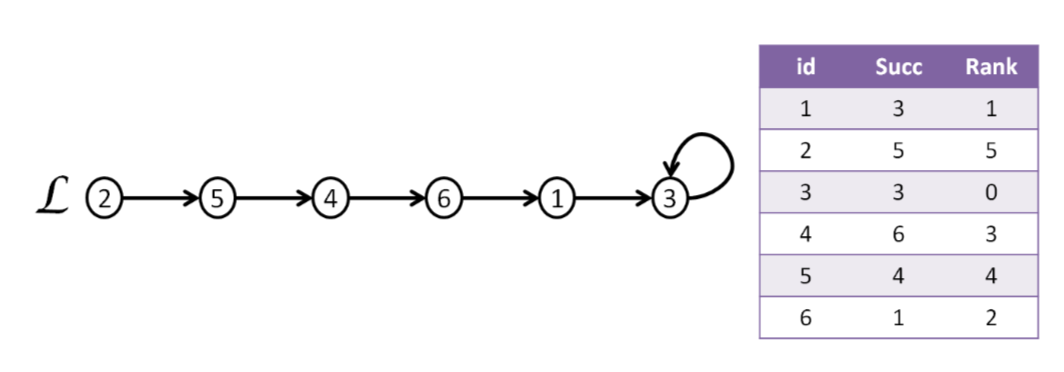
\includegraphics[width=\linewidth]{LinkedList.png}
 
\end{figure}

Ogni elemento della lista viene identificato con il suo id ovvero un intero che va da 1 a n. Per ogni elemento della lista manteniamo altre due informazioni, il rank e il successore.
L'ultimo elemento della lista ha come successore se stesso (viene creato un self-loop).
Ci sono tre metodi che possiamo utilizzare con il modello RAM per risolvere questo problema, questi metodi sfruttano l'accesso in memoria a costo costante:
\begin{itemize}
    \item Il primo metodo scorre la lista calcolando il numero (N) di elementi presenti al suo interno. Poi scorre di nuovo la lista e partendo dal primo elemento $i$ assegna il ranking $N-i$.
    \item Il secondo metodo crea un nuovo array di predecessori, in questo caso ogni elemento dell'array predecessori è nella forma $Pred[Succ(i)] = i$. Poi partendo dall'ultimo elemento assegno rank 0, poi 1, poi 2 ... poi assegno via via i vari rank.
    \item Un'ultima soluzione consiste nell'andare a calcolare il rank ricorsivamente. Il calcolo del rank viene svolto in questo modo: se $Succ[i] = i$ allora il $Rank(i)$ sarà pari a 0, altrimenti vado a calcolare ricorsivamente $Rank(i) = 1 + Rank(Succ(i))$
\end{itemize}

Questi metodi hanno una complessità che è O(n) ma il problema è legato al numero di operazioni I/O che vengono svolte perchè sono O(N) perchè l'accesso agli elementi non è continuo ma potrei saltare da una parte all'altra dell'array.
Quindi l'idea è quella di evitare di seguire i puntatori il più possibile per evitare alti costi per le operazioni di I/O.

\section{Tecnica del pointer Jumping}

La tecnica del pointer jumping consiste nell'utilizzo in parallelo di n processori che lavorano ognuno su un elemento della lista.
\begin{itemize}
    \item Ogni processore prende il suo elemento della lista e inizializza il rank a 0 se è l'ultimo elemento della lista mentre lo inizializza a 1 se è un elemento precedente.
    \item Ogni processore poi esegue le seguenti operazioni: prima calcola per il nodo i il rank corrispondente ovvero $Rank[i] += Rank[Succ[i]]$ poi calcola il successore del nodo i ovvero calcola $Succ[i] = Succ[Succ[i]]$.
\end{itemize}

Il valore del rank dei vari elementi della lista non cresce in modo lineare ma viene raddoppiato ad ogni step dell'algoritmo, questo vuol dire che la crescita è esponenziale e che il costo dell'esecuzione dell'algoritmo per ognuno degli n processori è $O(logn)$ in tempo. Complessivamente abbiamo un costo di $O(n*logn)$ operazioni svolte, perchè abbiamo n processori che svolgono $O(log n)$ operazioni.

\begin{figure}[h!]
  \centering
  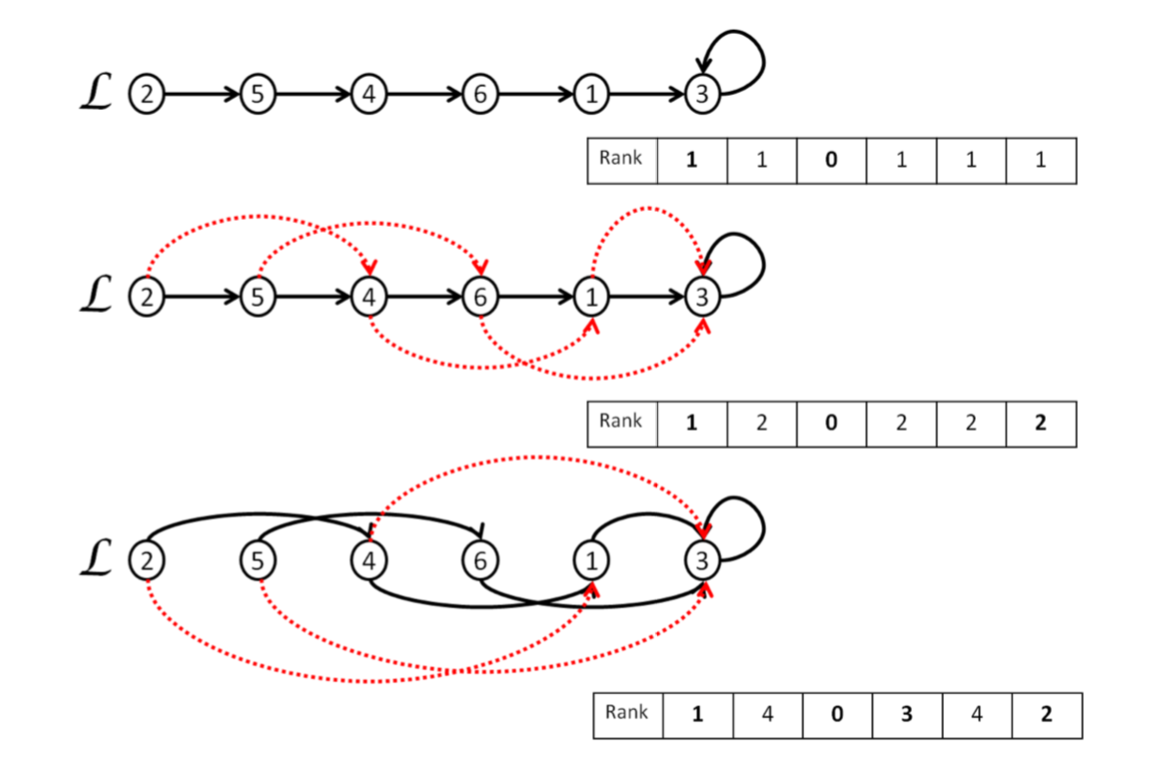
\includegraphics[width=\linewidth]{PointerJumping.png}
  
\end{figure}

\section{Simulazione dell'algoritmo con la memoria a 2 livelli}

Utilizzare la tecnica del Pointer Jumping nel modo in cui è stata descritta può comportare dei problemi per quel che riguarda il numero di operazioni I/O da effettuare perchè l'accesso in memoria può avvenire in modo totalmente random dato che gli elementi della lista non sono ordinati.
Per simulare il funzionamento delle due operazioni del pointer jumping (ovvero calcolo del successore e calcolo del rank) si usa il sorting e la scansione dell'array, il numero delle operazioni da effettuare è costante.
Le operazioni vengono simulate considerando la seguente forma $A[a_i]\ op\ A[b_i]$:
\begin{itemize}
    \item Nel caso dell'operazione di aggiornamento del rank l'"op" è la somma e l'assegnamento e A è l'array con i rank.
    \item Nel caso dell'operazione di ricerca del successore, op è l'operazione di assegnamento, A è l'array con i successori.
\end{itemize}

Questa operazione $A[a_i]\ op\ A[b_i]$ può essere eseguita in parallelo dagli n processori con un numero di operazioni di I/O pari a $O(\frac{n}{b})$, la simulazione consiste in 5 step:

\begin{itemize}
    \item Si crea per ogni elemento della lista una tripla in cui inseriamo $<a_i, b_i, 0>$ dove $a_i$ è l'id del nodo, $b_i$ è il successore e l'ultimo numero è il rank del nodo che, almeno all'inizio, viene settato a 0.
    \item Si fa un primo ordinamento delle triple basandoci sul secondo elemento.
    \item Si scorrono le triple e si creano delle nuove triple $<a_i, b_i, A[b_i]>$ dove $A[b_i]$ è il valore del rank del successore di $a_i$. (In questo caso l'operazione op è l'assegnamento perchè assegno il rank del successore).
    \item Si fa un secondo ordinamento basandoci sul primo elemento delle triple.
    \item Si fa la scansione delle triple e per ogni tripla si modifica il terzo valore andando a calcolare il nuovo rank (in questo caso è somma e assegnamento perchè sommiamo il rank che abbiamo con il rank del successore).
\end{itemize}

\textbf{Teorema: L'esecuzione in parallelo di n operazioni $A[a_i]\ op\ A[b_i]$ può essere simulata nella memoria a 2 livelli con un numero costante di scan e sort quindi abbiamo un numero di operazioni di I/O pari a $\frac{n}{B}$}
\newline \newline 
\textbf{Teorema: La simulazione dell'algoritmo del pointer jumping viene eseguita con la memoria a 2 livelli, sono necessari $O(log n)$ passaggi quindi il numero di operazioni di I/O da eseguire sono $\frac{n}{B}\ *\ logn $}.
\newline \newline 
\textbf{Teorema: Ogni algoritmo eseguito in parallelo su n processori che necessita di T step per terminare può essere simulato nella memoria a 2 livelli con un numero di operazioni di I/O pari a $\frac{n}{B}\ *\ T $}.
\newpage
Esempio di simulazione dell'algoritmo Pointer Jumping usando Scan e sort:

\begin{figure}[h!]
  \centering
  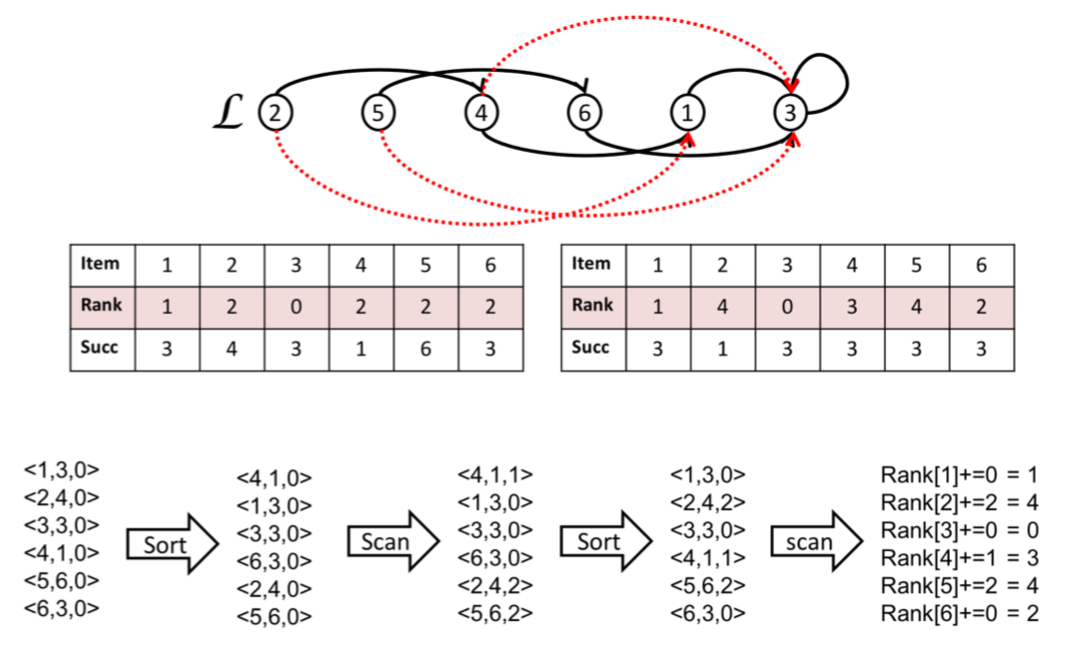
\includegraphics[width=\linewidth]{SimulazionePJ.png}
\end{figure}

\section{Approccio Divide & Conquer}



\fbox{\parbox{\dimexpr\linewidth-2\fboxsep-2\fboxrule\relax}{\begin{center}
    \textbf{Ripasso del Master Theorem}
    \end{center}
Il Master Theorem è il metodo che ci permette di risolvere le equazioni di ricorrenza del tipo: $T(N) = a\frac{n}{b} + f(n)$. Dove a indica il numero di sottoproblemi, $\frac{n}{b}$ indica la dimensione dei sottoproblemi e $f(n)$ indica il costo della divisione e della ricombinazione.
Nel Master Theorem abbiamo 3 casi differenti che vanno considerati per risolvere le equazioni di ricorrenza:
\begin{itemize}
    \item Calcoliamo $n^{log_b a - \epsilon}$, se $f(n)=O(n^{log_b a - \epsilon})$ ovvero $f(n)$ è minore allora la soluzione è $T(n) = \Theta(n^{log_b a })$.
    \item Calcoliamo $n^{log_b a - \epsilon}$, se $f(n)=\Theta(n^{log_b a - \epsilon})$ ovvero $f(n)$ è uguale allora la soluzione è $T(n) = \Theta(n^{log_b a }*log n)$.
    \item Calcoliamo $n^{log_b a - \epsilon}$, se $f(n)=\Omega(n^{log_b a - \epsilon})$ ovvero $f(n)$ è maggiore allora la soluzione è $T(n) = \Theta(f(n))$. Deve anche valere la condizione per cui $af(\frac{n}{b}) \leq c*f(n)$.
\end{itemize}
}
}
\newline\newline
Per risolvere il problema del List Ranking possiamo utilizzare un approccio ricorsivo che quindi consiste nel suddividere il problema nella fase di "Divide" andando poi a risolvere ricorsivamente il problema sul set di dati ridotto nella fase di "Conquer", alla fine nella fase di "Recombine" vengono ricombinate le soluzioni dei sottoproblemi.
Nel caso del problema del List Ranking le fasi sono le seguenti:

\begin{itemize}
    \item Divide: Creiamo un set I di elementi presi dalla lista iniziale, il set I deve essere tale che per ogni elemento presente in I, il successore dell'elemento non viene inserito nel set I. Questo vuol dire che la lunghezza del set I sarà $|I| \leq \frac{n}{2}$ e sarà $|I| > \frac{n}{c}$. Dove $c>2$.
    \item Conquer: Partendo dalla lista iniziale eliminiamo gli elementi che sono presenti in I e creiamo una seconda lista L'. Per ogni elemento x presente nella lista tale che $Succ[x]$ è presente in I dobbiamo andare a calcolare: $Rank[x] += Rank[Succ[x]]$ e poi $Succ[x] = Succ[Succ[x]]$. In questo modo il $Rank[x]$ indicherà per ogni x nella nuova lista la distanza tra x e il successore attuale di x.
    \item Recombine: in questa fase abbiamo calcolato il rank di tutti gli elementi presenti nella lista che abbiamo creato togliendo gli elementi del set I. Per ogni elemento x che appartiene a I dobbiamo andare a calcolare $Rank[x] = Rank[x] + Rank[Succ[x]]$ dove $ Rank[Succ[x]]$ indica la distanza tra il successore di x e la fine della lista ed è disponibile perchè l'abbiamo calcolato in precedenza dato che Succ[x] sta sicuramente nella lista L' che abbiamo creato.
    Mentre $Rank[x]$ indica la distanza tra x e il successore nella lista di partenza.
\end{itemize}

Un esempio:

\begin{figure}[h]
  \centering
  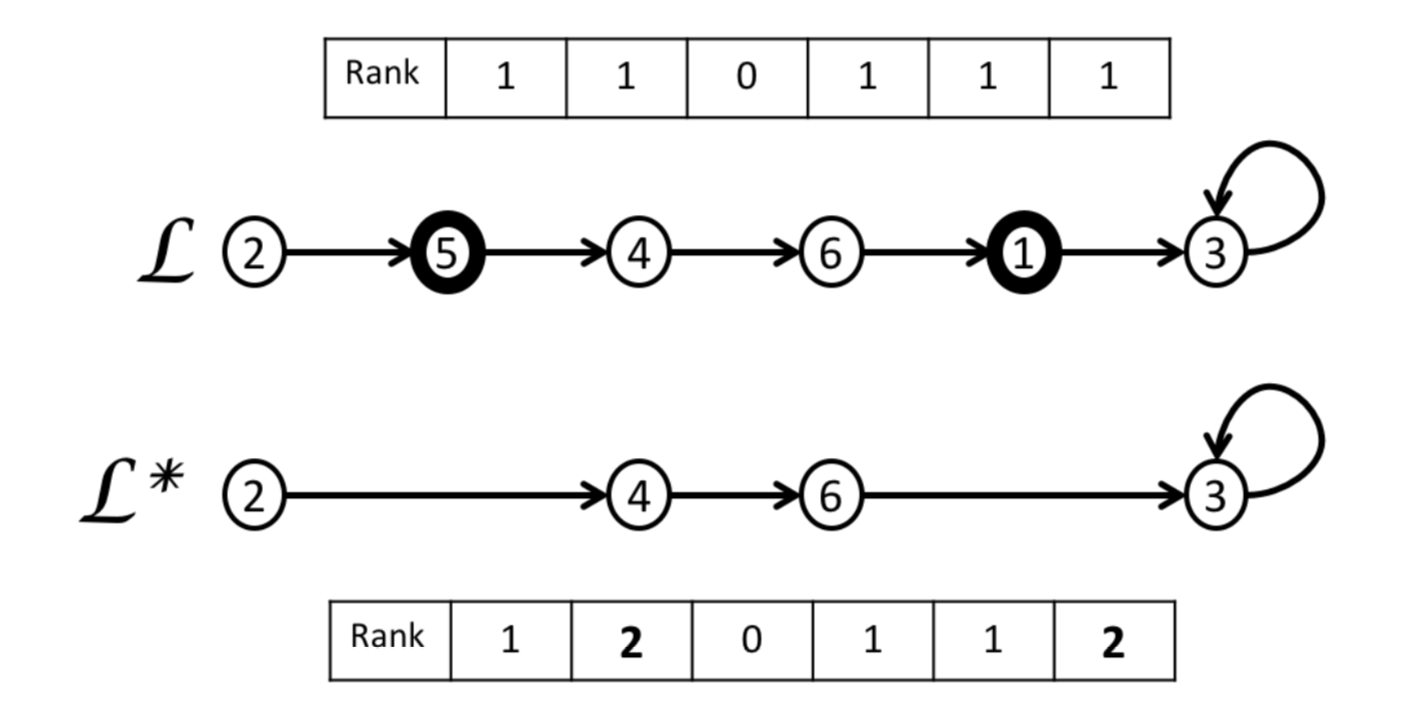
\includegraphics[width=0.8\linewidth]{ListRankingRec.png}
\end{figure}

Analizzando l'algoritmo, per capire il numero di operazioni I/O che vengono effettuate dobbiamo prendere in considerazione le tre fasi, divide, recombine e conquer.
In particolare per la fase di divide abbiamo un costo $I(n)$ che dipende dal modo in cui creiamo il set I. 
Per la fase di recombine abbiamo un costo che è $O(\frac{n}{b}$ e per la fase di conquer consideriamo il numero di elementi che rimangono nella lista L' ovvero $T((1-\frac{1}{c})n)$.
Quindi nel complesso abbiamo che il numero di operazioni di I/O viene indicato dalla seguente equazione di ricorrenza:
$T(n) = I(n) + O(\frac{n}{b} + T((1-\frac{1}{c})n)$.
Ora il problema sta nel modo in cui creiamo I perchè se scorriamo la lista e scegliamo se inserire o no l'elemento abbiamo un costo enorme in termini di I/O, quindi si deve trovare una alternativa.

\section{Coin Tossing}

\subsection{Coin Tossing randomizzato}

L'idea del coin tossing è che per ogni elemento della lista viene lanciata una monete, se esce testa e sull'elemento successivo esce croce allora vuol dire che posso selezionare l'elemento. Abbiamo 4 possibili configurazioni di testa e croce, quindi al più in I finiscono $\frac{n}{4}$ elementi.
Per il teorema che dice che l'esecuzione parallela su n processori può essere simulata con un numero costante di scan e sort con un numero di operazioni I/O pari a $\Theta(\frac{n}{b})$ allora possiamo dire che la I(n) di prima mi costa $\Theta(\frac{n}{b})$ al caso pessimo quindi possiamo riscrivere l'equazione di ricorrenza:
$T(n) = O(\frac{n}{b} + T(\frac{3n}{4})$.
Il $T(\frac{3n}{4})$ esce fuori perchè $I=\frac{1}{c}*n$ quindi L' diventa $|L'| = n - \frac{n}{c}$, se c=4 allora abbiamo che $|L'| = \frac{3}{4}$.
Risolvendo l'equazione (siamo nel caso 3) possiamo vedere che il list ranking utilizzando la procedura ricorsiva mi costa $O(\frac{n}{b})$.

\subsection{Coin Tossing Deterministico}

Con il coin tossing deterministico la procedura è differente e prevede vari step:

\begin{itemize}
    \item Per ogni elemento [1,n] della lista assegnamo un valore coin(i) pari a i-1. Quindi da 0 a n-1. Per rappresentare questo valore di coint(i) mi bastano $b = log n$ bit, per ogni elemento $bit_b$ indica questo valore del coin.
    \item Ora vogliamo passare da n valori del coin a 6 valori, per farlo:
        \begin{itemize}
            \item Per ogni i nella lista controlliamo $bit_b(i)$ e $bit_b(succ[i])$. Calcoliamo $\Pi(i)$ ovvero la posizione in cui i due valori differiscono e calcoliamo $z(i)$ ovvero il valore di $bit_b(i)$ che differisce rispetto a $bit_b(succ[i])$.
            \item Ora assegnamo $coin(i) = 2*\Pi(i) + z(i)$. Quindi ora mi bastano solamente $log(b) + 1$ bit per rappresentare il coin di i. 
        \end{itemize}
    \item Ora da 6 valori di coin vogliamo passare a 3 valori di coin. Per farlo consideriamo tutti gli elementi della lista che hanno un valore di coin compreso tra 3 e 5.
    Modifichiamo il loro valore di coin, $coin(i) = {1,2,3} - {Coin(pred(i)), Coin(succ(i))}$.
    \item Ora possiamo selezionare gli elementi di I, prendiamo tutti gli elementi tali che $coin(i) < coin(succ(i))$ e  $coin(i) < coin(pred(i))$.
\end{itemize}

Ci sono alcune cose da notare che fanno funzionare l'algoritmo:
\begin{itemize}
    \item È importante notare che non è possibile che i coin di due elementi vicini siano uguali, questo è fondamentale per l'ultimo passaggio ma anche per dimostrare la correttezza dello step in cui passiamo da 6 a 3 valori. Questa cosa non è possibile perchè se lo fosse avremmo $\Pi(i)+z(i) = \Pi(succ(i))+z(succ(i))$, quindi vorrebbe dire che $\Pi(i) = \Pi(succ(i))$ e questo implicherebbe l'assenza di differenze tra $bit_b(i)$ e $bit_b(succ(i))$. 
    \item Per quanto riguarda la complessità in termini di operazioni I/O, per passare da n valori di coin a 6 valori di coin, ogni volta ho una applicazione del logaritmo, quindi in pratica dobbiamo capire quante volte si effettua l'operazione del passaggio da n a 6 valori. Dato che la riduzione è logaritmica possiamo dire che vengono effettuate $log*n$ iterazioni. Vuol dire che applico * volte il logaritmo.
    Quindi ci metto poche iterazioni per passare da n a 6, quindi possiamo dire che per formare il set I abbiamo bisogno di $O(\frac{n}{b}*log*n)$, dato che $log*n$ cresce molto lentamente, possiamo considerarlo come una costante quindi abbiamo un numero di operazioni di I/O pari a $O(\frac{n}{b})$.
\end{itemize}

Quindi alla fine anche il coin tossing deterministico risolve il problema del list ranking con un numero di operazioni I/O che al caso pessimo saranno $O(\frac{n}{b})$.
Quindi questo è il caso migliore perchè abbiamo il caso pessimo e una situazione deterministica.

\chapter{Lezione 5: Ordinamento di array con elementi atomici}

In questo caso il problema è quello del sorting, abbiamo un array S con n elementi atomici e dobbiamo ordinarlo in modo crescente.
Con elementi atomici indichiamo quegli elementi che occupano un numero costante di celle di memoria.
C'è un altro problema che è legato al sorting, si tratta del problema del "permuting", in questo caso abbiamo un array S di n elementi e poi abbiamo un array $\Pi$ che mi indica la permutazione delle posizioni dell'array S di partenza. L'obiettivo è permutare gli elementi dell'array S andando a considerare l'ordinamento che viene indicato nell'array $\Pi$.
Nel modello Ram abbiamo che l'ordinamento costa in termini di tempo $O(nlogn)$ mentre la permutazione costa $O(n)$.
Se però pensiamo al modello con 1 disco e una memoria interna dobbiamo pensare al costo in termini di operazioni I/O che dobbiamo effettuare. In questo caso il vero problema è legato non al sorting dei dati quanto invece all'accesso ai dati, abbiamo quindi un I/O Bottleneck. Permutare gli elementi di un array con un modello con 1 disco mi comporta un numero di accessi al disco (Operazioni I/O) che è $O(n)$ e soprattutto che non è per niente efficiente perchè carico un blocco e poi accedo magari solamente ad un elemento del blocco sfruttando quindi solamente $\frac{1}{B}$ del blocco.

\section{Il Merge Sort}

Vogliamo considerare l'esecuzione dell'algoritmo Merge Sort nel modello con una memoria esterna da cui leggiamo blocchi di dati di dimensione B e una memoria interna di dimensione M.
Il Merge sort è un algoritmo Divide et Impera, il codice:

\begin{code}
\begin{lstlisting}[escapeinside={(*}{*)}]
MergeSort(S,i,j):
    if(i<j):
        m = (i+j)/2
        MergeSort(S,i,m-1)
        MergeSort(S,m,j)
        Merge(S,i,m,j)
\end{lstlisting}
\end{code}

Nel codice abbiamo un primo controllo iniziale, con l'if controlliamo di avere un array di dimensione maggiore di 1 elemento. Poi abbiamo le due chiamate ricorsive a MergeSort che contribuiscono a suddividere il problema in due sottoproblemi generando due array. Il numero complessivo delle chiamate ricorsive che vengono effettuate è $O(log n)$ perchè ogni volta la dimensione dell'array da ordinare viene divisa in 2.
La chiamata Merge invece serve per unire i due sotto array, per svolgere questa unione utilizziamo due puntatori che utilizziamo per confrontare i due elementi dell'array, il costo della procedura Merge è $O(n)$. Quindi nel complesso il costo è $O(nLogn)$.
Alla fine l'array ordinato non è quello iniziale ma ne abbiamo uno nuovo, quindi la complessità in spazio è $O(n)$ e l'ordinamento non viene eseguito in-place.

La situazione si fa più complicata quando l'array da ordinare non entra completamente nellla memoria interna di dimensione M ovvero quando $n>M$.
In questo caso va considerato più di tutti il costo necessario per svolgere le operazioni di I/O.
Per calcolare il numero delle operazioni I/O che dobbiamo eseguire vanno considerati i seguenti aspetti:
\begin{itemize}
    \item Ammesso di avere una memoria interna M che ci permette di mantenere almeno due pagine di dimensione B ($M \geq 2B$), consideriamo il Merge, abbiamo due sotto array di dimensione x e dobbiamo andare a unire questi sotto array ordinati in un unico array.
    Il numero di operazioni di I/O in lettura per eseguire il merge sono $O(x/B)$ per il primo sotto array e altrettanti per il secondo. Quindi nel complesso abbiamo $O(x/B)$ operazioni di I/O.
    Per la scrittura il discorso è simile, devo scrivere nell'array destinazione x elementi che sono posizionati in modo contiguo quindi avremo sempre un numero di operazioni I/O pari a $O(x/B)$.
    Quindi complessivamente la complessità del Merge Sort la possiamo indicare con la seguente equazione di ricorrenza: $T(N) = 2T(\frac{n}{2}) + O(\frac{n}{b})$ quindi il costo del Merge Sort è $O(\frac{n}{B}Logn)$.
    \item Nella prima parte del ragionamento non abbiamo considerato una cosa importante, ad un certo punto dividendo l'array arriveremo ad un sotto array di dimensione $z = O(m)$ che quindi mi costa $O(z/B)$ operazioni di I/O per essere caricato in memoria ma poi non mi costa ulteriormente perchè è tutto in memoria e non devo fare altre operazioni di I/O.
    Questa idea la posso applicare su un numero di sotto array pari a $O(n/M)$. 
    Questo comporta che al costo di $O(\frac{n}{B}Logn)$ che avevo in precedenza per le operazioni di I/O (che era derivato dal fatto che ho Logn passaggi di divisione) devo andare a togliere il numero di step che verrebbero fatti dal momento in cui i dati entrano totalmente in memoria ovvero $O(\frac{n}{B}LogM)$.
    Quindi complessivamente abbiamo $O(\frac{n}{B}Logn) - O(\frac{n}{B}LogM)$ ovvero un numero di operazioni I/O pari a $O(\frac{n}{B}Log\frac{n}{M})$.
\end{itemize}

\subsection{Come migliorare il Merge Sort}

Abbiamo detto che il numero di operazioni di I/O che svolge il Merge Sort se l'array da ordinare non entra tutto in memoria è $O(\frac{n}{B}Log\frac{n}{M})$.
Sarebbe più corretto scrivere che il numero di operazioni di I/O è $O(\frac{n}{B}Log\frac{n}{cM})$ dove la c è uguale a 1 nel caso dell'heap sort perchè l'ordinamento viene effettuato in place, è poco meno di 1 nel caso del quick sort per via delle chiamate ricorsive mentre è 0.5 nel caso del Merge Sort perchè devo anche mantenere un array in cui inseriamo i valori ordinati.
Quindi per diminuire il numero di operazioni da effettuare o aumentiamo la dimensione di B, o aumentiamo la dimensione di M oppure cambiamo il valore del 2 del logaritmo.
Ci sarebbe anche la possibilità di andare ad comprimere i run ordinati utilizzando il gap encoding e poi qualche algoritmo di compressione di interi, in questo modo in memoria entrano più elementi di S.

Ci sono due possibili soluzioni che possono essere adottate.

\subsubsection{Snow Plow}

È un metodo che è stato proposto da Knuth, noi sappiamo che nel merge sort creiamo n/M blocchi ordinati e per ordinarli non abbiamo costi di I/O perchè sono grandi M ed entrano in memoria interna.
L'idea è quella di aumentare virtualmente M andando a creare dei run ordinati di dimensione 2M. In questo modo riduciamo la profondità a cui si arriva (e che comporta operazioni di I/O) che quindi non sarà più $log(\frac{n}{M})$ ma $log(\frac{n}{2M})$.
La tecnica Snow Plow permette di aumentare virtualmente la memoria interna di un fattore 2 (in media) quindi alla fine avremo un numero di operazioni di I/O pari a $O(\frac{n}{B}(log(\frac{n}{2M}))s$.

L'algoritmo utilizza:
\begin{itemize}
    \item Tutta la memoria interna di dimensione M
    \item All'interno della memoria M viene creato un Min-Heap H (che non consuma spazio)
    \item Viene utilizzato un array U.
\end{itemize}

L'algoritmo funziona in questo modo:

\begin{itemize}
    \item Nella prima fase andiamo a prendere M elementi dall'array S da ordinare e li inseriamo nel Min Heap H.
    \item Ora entriamo in un while, fino a quando il Min-Heap non è vuoto, estraiamo il minimo da H e lo scriviamo nel run in output, poi prendiamo un elemento da S, se è maggiore del minimo estratto lo mettiamo nello heap, altrimenti nell'array U.
    \item Quando si svuota il Min-heap vuol dire che invece U sarà pieno, ci saranno M elementi, a questo punto ricominciamo dal punto precedente andando a inserire gli elementi di U nello heap e rientriamo poi nel while.
\end{itemize}

Il codice completo è il seguente:

\begin{code}
\begin{lstlisting}[escapeinside={(*}{*)}]
H = Creare un Min Heap partendo dall$'$array U
U = vuoto
while(H non vuoto):
    Min = Estrai il minimo da H
    Scrivi min sul run in output
    prendi un elemento x da S
    if(x < min):
        Add x to U
    else:
        Add x to H
\end{lstlisting}
\end{code}

Ora bisogna considerare quanto scrivo in output e quanto leggo da S prima che si svuoti il Min Heap.
\begin{itemize}
    \item Diciamo che leggiamo da S un numero di elementi pari a $\tau$, quindi vuol dire che di questi elementi almeno M devono andare a finire in U
    \item Quindi in H ci finiscono $\tau - M$ elementi
    \item Vuol dire che in output, per ogni run ci finiscono M elementi che stavano già nello heap più $\tau - M$ elementi che ho inserito. Ovvero ci finiscono $\tau$ elementi.
    \item Se consideriamo che gli elementi di S hanno una probabilità uniforma di essere minori del minimo dello heap o di essere maggiori, allora possiamo dire che $\frac{\tau}{2}$ elementi letti da S finiscono in H e $\frac{\tau}{2}$ finiscono in U.
    \item Dato che sappiamoc che in U ci devono finire M elementi possiamo dire che $\frac{\tau}{2} = M$ Ovvero  $\tau = 2*M$.
    Quindi leggiamo $\tau = 2*M$ elementi da S.
\end{itemize}

Cosiderando tutto questo possiamo dire che utilizzando Snow Plow, verranno creati un numero di run ordinati pari a $O(\frac{n}{M}$ ma ognuno di questi run sarà più lungo di M, in media sarà $2M$. Quindi in pratica ora non devo arrivare fino ai run lunghi M per non avere più operazioni di I/O ma mi basterà arrivare ai run grandi 2M.
Quindi la complessità in termini di I/O del Merge sort utilizzando Snow Plow diventa in media $O\frac{n}{b}log(\frac{n}{2M})$.

\section{Multi Way Merge Sort}

Con Snow Plow siamo passati ad una complessità delle operazioni di I/O del Merge Sort che è (nel caso del 2 disk level) in media $O\frac{n}{b}log(\frac{n}{2M})$. Ovvero abbiamo raddoppiato "virtualmente" la dimensione di M.

Nel MultiWay Merge Sort invece si lavora sulla base 2 del logaritmo.
Quando facciamo il merge dei vari run, con il classico Merge Sort andiamo a prendere due run alla volta e facciamo il merge, vuol dire che in memoria ci troviamo solamente due blocchi per leggere e uno per scrivere mentre tutto il resto rimane inutilizzato.
In pratica in memoria potremmo tenere un numero di blocchi per leggere $k = M/B\ -\ 1$ e invece ne teniamo solamente 2.
L'idea quindi è quella di andare ad aumentare il numero dei blocchi che sono presenti in memoria e da cui vogliamo prendere elementi da mergiare. In particolare dato che vogliamo inserire k blocchi, vorremo confrontare k elementi (1 per ogni blocco) e restituirli in output.

L'idea è di utilizzare un Min Heap, carichiamo k blocchi in memoria interna e poi leggiamo il primo elemento dei k blocchi e lo inseriamo all'interno del Min Heap.
Per ogni elemento del Min Heap non ci salviamo solamente il suo valore ma anche il run da cui proviene, in questo modo quando estraiamo il minimo dal Min Heap per metterlo in output, potremo andare nel run corrispondente per estrarre un altro elemento da quello specifico run. Il processo di merging richiede un tempo $O(log k)$ per ogni singolo elemento e poi, presi k run la cui lunghezza è pari a z richiede un numero di operazioni di I/O pari a $O(z/B)$.
In questo modo riusciamo ad aumentare il 2 della base del logaritmo che diventa $M/B$ perchè ora non uniamo più due run alla volta ma $k = M/B -1 $.
Quindi complessivamente il Multi Way Merge Sort richiede una compelessità in termini di tempo pari a $O(nlogn)$, il numero di operazioni di I/O però scende a $O(\frac{n}{b}log_{\frac{M}{B}}\frac{n}{M})$.


\section{Lower Bound}

Consideriamo due problemi, il sorting e il permuting. 
Nel Ram model possiamo dire che il lower bound del sorting è $\Omega(nLogn)$ mentre il permuting è $O(n)$ perchè faccio degli spostamenti accedendo in memoria e gli accessi però non li pago.
Ora consideriamo il 2 disk model, in questo caso il numero di operazioni I/O che pago per il sorting è identico al numero di operazioni I/O che pago per il permuting, questo vuol dire che abbiamo un collo di bottiglia per quel che riguarda lo spostamento dei dati nel disco e non nel sorting.

Per la soluzione del problema del permuting abbiamo due metodi nel caso del 2-disk model:
\begin{itemize}
    \item Simuliamo quello che succede nel modello ram ovvero abbiamo la lista S, la lista delle permutazioni $\Pi$ e poi creiamo la lista S' andando a mettere in ogni posizione i di S' l'elemento $S[\Pi[i]]$.
    Questo mi costa $O(n)$ operazioni di I/O.
    \item Possiamo usare il sorting per risolvere il problema del permuting. Si fa così:
        \begin{itemize}
            \item Creiamo una sequenza di coppie $<i, \Pi[i]>$ dove i è la posizione in cui $S[\Pi[i]]$ deve essere posizionato
            \item Si fa un primo sort sul secondo elemento della coppia.
            \item Si fa una operazione di Scan sostituendo $\Pi[i]$ con $[\Pi[i]]$
            \item Si fa un sort sul primo elemento delle coppie
        \end{itemize}
    L'algoritmo fa due ordinamenti e una scansione, tutto questo mi costa un numero di I/O pari a $O(\frac{n}{B}log_{\frac{M}{B}\frac{n}{m}})$.
    
\end{itemize}
Quindi in generale l'operazione di permuting nel 2 level model mi costa un numero di I/O pari a $min(n,\frac{n}{B}log_{\frac{M}{B}\frac{n}{m}})$.


\subsection{Lower Bound per il sorting con modello RAM}

Per calcolare il lower bound del sorting nel modello Ram dobbiamo utilizzare un albero di decisione, in ogni nodo dell'albero viene presa una decisione e ogni nodo poi ha due figli. Quindi l'albero è binario e se abbiamo n elementi da ordinare avremo $n!$ possibili ordinamenti che quindi corrispondono a $n!$ foglie dell'albero.
Ogni path dal nodo root ad una foglia è una possibile computazione.
Se l'albero ha altezza h vuol dire che all'ultimo livello dell'albero dovremo avere $n!$ foglie, quindi:
\begin{equation}
    2^h \geq n! => h \geq log n! => h \geq n log n
\end{equation}
L'ultimo passaggio lo possiamo fare per l'approssimazione di Stirling. Quindi il lower bound nel ram model è $\Omega(nlogn)$

\subsection{Lower Bound per il sorting con 2 Level Model}

Anche in questo caso dobbiamo sempre considerare l'albero di decisione in cui ogni nodo è un confronto e una operazione di I/O. Il numero delle foglie è sempre $n!$. 
La differenza rispetto al modello ram è il numero di figli di ogni nodo (fan-out), un solo I/O legge B elementi e ce ne sono già M-B in memoria, questo I/O mi genera un numero di possibili ordinamenti differenti dei B elementi che è pari a $\binom{M}{B}$ modi differenti, vanno però considerate anche le possibili permutazioni di B che sono $B!$ quindi il fan out dei nodi è $(\binom{M}{B})B!$.
Va considerato anche un altro dettaglio però, dopo aver fatto O(n/b) I/O avremo già considerato tutti gli elementi una volta, quindi non è necessario considerare le possibili permutazioni di B quindi per alcuni livelli dell'albero di decisione il fan out dei nodi sarà $(\binom{M}{B})$.

Se consideriamo un percorso root-foglia lungo t avremo $\frac{n}{b}$ nodi che avranno un fan out $(\binom{M}{B})B!$ e $t-b$ nodi che invece avranno un fan out $(\binom{M}{B})$.
Quindi il numero delle foglie dell'albero sarà:
\begin{equation}
    ((\binom{M}{B})B!)^{\frac{n}{B}} * (\binom{M}{B})^{t-\frac{n}{B}} 
\end{equation}

Questo va posto sempre maggiore o uguale a $n!$ perchè il numero di foglie deve essere quello quindi abbiamo:

\begin{equation}
    ((\binom{M}{B})B!)^{\frac{n}{B}} * (\binom{M}{B})^{t-\frac{n}{B}} \geq n! = (\binom{M}{B})^{t}*(B!)^{\frac{n}{B}}\geq n!
\end{equation}
\begin{equation}
    t Log(\binom{M}{B}) * \frac{n}{B}Log(B!) \geq Log n!
\end{equation}
\begin{equation}
    t Log(\binom{M}{B}) * B\frac{n}{B}Log(B) \geq nLog n
\end{equation}
\begin{equation}
    t Log(\binom{M}{B}) * n Log(B) \geq n Log n
\end{equation}
\begin{equation}
    t Log(\binom{M}{B}) \geq n Log n - n Log(B)
\end{equation}
\begin{equation}
    t Log(\binom{M}{B}) \geq n Log \frac{n}{B}
\end{equation}

Con la formula del cambio di base:

\begin{equation}
    t \geq \frac{n}{B} Log_{\frac{M}{B}} \frac{n}{B}
\end{equation}

Quindi vuol dire che il numero di operazioni I/O da eseguire è pari a $\frac{n}{B} Log_{\frac{M}{B}} \frac{n}{B}$.
Se abbiamo invece D dischi diventa $\frac{n}{DB} Log_{\frac{M}{B}} \frac{n}{DB}$.


\subsection{Lower bound per le permutazioni (SENZA DIMOSTRAZIONE)}

Nel caso delle permutazioni il lower bound è $\Omega(n)$ se $B*log(\frac{M}{B})\leq logn$.
Altrimenti è $\Omega(\frac{n}{B}Log_{\frac{M}{B}}\frac{n}{M})$

\section{Distribution Based sorting paradigm}

Il Quick Sort è un altro algoritmo di ordinamento che è sempre ricorsivo come il Merge Sort ma non ha lo step di recombine perchè l'ordinamento viene effettuato in-place e soprattutto l'efficienza dell'algoritmo dipende dal modo in cui viene suddiviso l'array su cui vengono poi effettuate le chiamate ricorsive.
Il codice di QuickSort:
\begin{code}
\begin{lstlisting}[escapeinside={(*}{*)}]
QuickSort(S,i,j):
    if(i<j):
        r = posizione del pivot che scelgo
        inverti S[r] con s[i]
        p = partition(S,i,j)
        QuickSort(S,i,p-1)
        QuickSort(S,p+1,j
\end{lstlisting}
\end{code}

La chiave del Quick Sort è l'utilizzo di un pivot e della procedura partition che divide l'array in due parti, una parte contiene gli elementi dell'array minori del pivot e una parte gli elementi dell'array maggiori del pivot.
La scelta del pivot è importante perchè più riusciamo a creare due sub array bilanciati su cui fare la ricorsione e più abbiamo la possibilità di raggiungere una complessità in termini di tempo pari a $O(nLogn)$ così come avviene nel Merge Sort, nel caso pessimo (un sub array enorme e uno vuoto) abbiamo invece una complessità pari a $O(n^2)$.
Per migliorare il QuickSort proviamo a modificare il modo in cui si effettua il partizionamento dell'array.

\subsection{3 Way Quick Sort}

\end{document}